\section{Virtual Observatory by Region}
\label{sec:vo_services}

The IVOA architecture only defines a general framework and
standards that their members should follow, but each VO develop
their own services and tools depending on their specific goals.
The founders and first members are the same countries that have
been developing astronomy and astronomical instruments in the world,
such as in Western Europe, North America, east Asia and Oceania. During the last
few years,
new VOs in other regions were integrated to IVOA, specially in the southern
hemisphere, like the two youngest members: South Africa and Chile.
This offers not only a better worldwide coverage, but the chance of
better exploiting the high-quality data produced by observatories
located in those countries, both locally and globally.

\begin{figure}%[h]
\begin{center}
   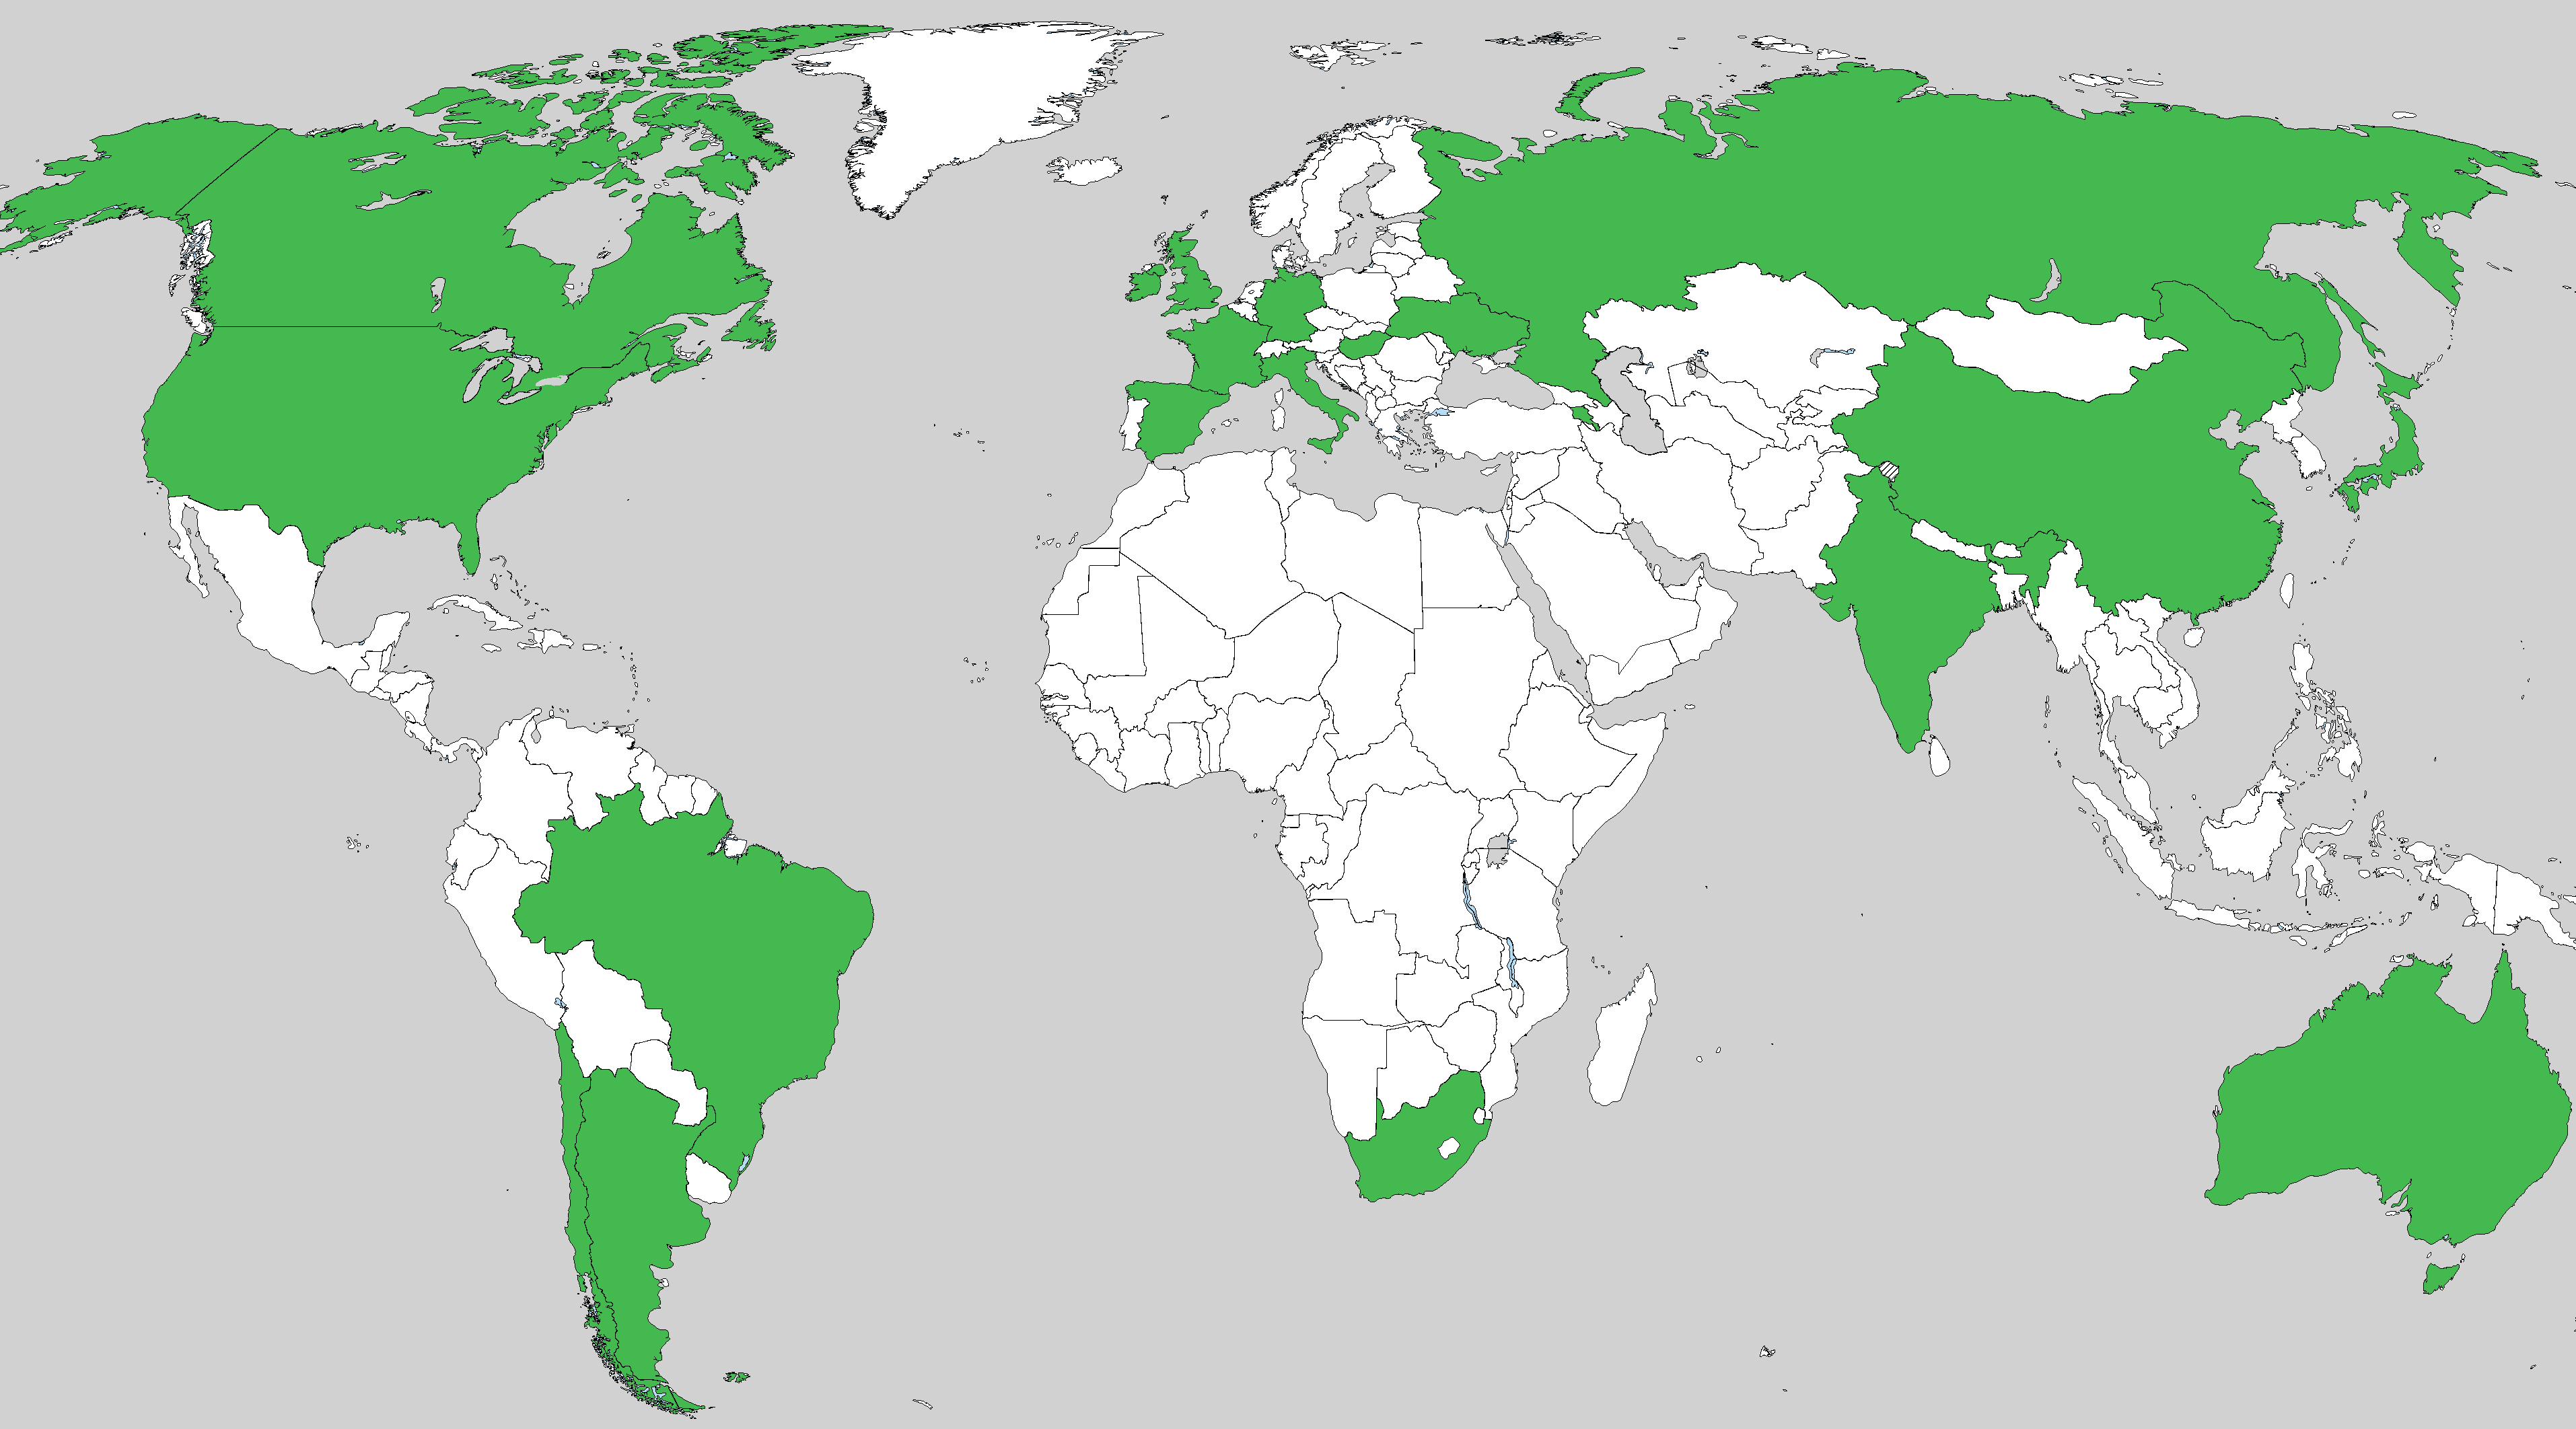
\includegraphics[width=0.9\linewidth]{img/VO-worldwide.png}
   \caption{International Virtual Observatory Alliance presence in the world.}
\label{figure:worldview}
\end{center}
\end{figure}

In the rest of this section, the VO initiatives are briefly
described by region (see Figure~\ref{figure:worldview}) to grasp the idea of the advances of
the VO, yet not all of them are included due to space 
constraints.

\subsection{North America}

The \textbf{Canadian Virtual Observatory} (CVO) has largely focus on the CANFAR Virtual Storage
System, which
allows accessing very large resources for both storage and processing, 
using a cloud based framework \cite{Gaudet2011}. 
This is a very generic framework for accessing and processing 
large astronomical data sets that implements most of the
VOSpace standard of IVOA \cite{Graham2007a}. CVO also has implemented
IVOA's data access services like TAP for metadata queries 
and SIA for image access.

A central objective of any VO is to make data accessible by astronomers,
for which the \textbf{US Virtual Astronomical Observatory} (US-VAO) 
offers a web-based service called Data Discovery Tool 
that retrieve data contained in the VO~\cite{McGlynn2013}. 
As a complement, a specific service for discovering time-series data
is also available, called Time Series Search Tool \cite{Graham2012}.
In terms of cloud data processing, the NVO has a Cross-Comparison Tool 
which perform fast positional cross-matches between a large number of 
sources, and a tool for researching multiple sky positions simultaneously (VIM)
\cite{Hanisch2012}.
It also offers a user-side application to find, plot and fit the
Spectral Energies Distributions (SEDs), called Iris~\cite{Laurino2013}.

\subsection{Europe}

One of the most mature VO is \textbf{Astrogrid} (United Kingdom)
\cite{Lawrence2002}, which implements
several IVOA-compliant services and offer very popular user applications
for accessing the VO services~\cite{Lawence2009}.
The implemented services are: \emph{Registry}
for discovering VO services, \emph{Community} to manage user accounts, 
\emph{VOSpace} for virtual file systems and processing, \emph{CEA} for running
generic asynchronous user applications, and \emph{DSA} for metadata/database
access. The very successful stand-alone applications of Astrogrid are 
the VODesktop~\cite{Tedds2008} for data and
TOPCAT \cite{Graham2007} for metadata.
Between other initiatives, Astrogrid offers a middleware platform 
that offers an API for accessing VO services, and a specific 
library for Python scripting.

The \textbf{German Astrophysical Virtual Observatory} (GAVO) is other important VO in Europe that focuses not
only in observational data, but also in theoretical data \cite{Lemson2007}.
The GAVO Data Centre is the service that implements several IVOA standards for 
accessing to the ROSAT archive and other data, for example 
\emph{Registry}, \emph{SIAP}, \emph{SCS}, \emph{VOTable}, \emph{VOPlot}, 
\emph{TAP}, \emph{SSAP}, etc. The services for 
theoretical data includes access to the MultiDark Simulation Database, %\cite{}
% Search
MPA Simulations, %\cite{},
% search
RAVE, % \cite{},
% search
Millenium data, % \cite{},
% search
and TheoSSA, % \cite{}.
% search
Moreover, GAVO offers a full distribution of their server software, called
DaCHS, and maintains SPLAT (a VO-enable spectral analysis tool) and the command line TAP
client \texttt{tapsh}.


The data access services of the \textbf{Observatoires Virtuels France}
(VO-France) are mainly concentrated in the 
CDS Portal, which is a mature service that host popular web-based and
user applications such as Simbad, Aladin, Vizier, Sesame, SimPlay, X-match,
etc., following the IVOA standards. 
Just to highlight a few, Sesame is a name service that query to 
three very complete catalogs and object databases (Simbad, Vizier and Ned),
in order to resolve a name into RA/DEC coordinates. Other interesting 
service is X-match which performs a cross-matching between large amount
of CDS objects or uploaded ones using a grid-based platform.
%search
Another recent VO-France project that is not part of CDS Portal 
is GhoSST, % \cite{},
%search,
which is an experimental database on spectroscopy of solids, that
plans in the near future to be IVOA compliant.

The \textbf{Italian Virtual Observatory} (VObs.it) provides data access to
their archives through the VO-Dance service \cite{Smareglia2001},
which implements several IVOA standards and provides a user-friendly procedure 
to publish astronomical data. An interesting service that VObs.it offers is
VODKA (VO Data Keeping-up Agent), which is a ``new VO actor which monitors the
state of the VO seeking for changes in services and datasets and notifying users
for those changes and updates''. \cite{Laurino2011}

Even though the \textbf{Spanish Virtual Observatory} (SVO) is a younger VO
compared to the previous ones, it
provides access to numerous databases of observational data, and also manages a
theoretical database of synthetic spectra, models and even asteroseismology.
Between the offered IVOA-compliant services we found the VO SED Analyzer (VOSA)
for comparing, managing and processing user or VO photometry-tables,
%search
and the VOSED, which is a SED generator using the VO data.
%search
Also, they provide other interesting services like the Filter Profile Service
database, and the TESELA service \cite{Cardiel2011} to access a catalog 
of blank regions.
The SVO is moving also to data mining projects like the automated classification
of light curves, and the GAIA project that aims to produce a 3D chart of the 
Milky Way. 

The \textbf{Hungarian Virtual Observatory} (HVO) offers a web-based Spectrum
Service \cite{Dobos2006},
that allows access, manipulation and composition of
several measured spectra of astronomical objects. It
also plan to include synthetic spectra generated by
astrophysical models that can be compared with observational
data. Other future plans are automatic photometric redshift 
estimation and performing all these computations in grid clusters. 

The \textbf{Ukrainian Virtual Observatory} (UkrVO)
offers access to the data generated by several Ukranian observatories 
through the Joint Digital Archive (JDA) service. Some of these archives 
(such as DBGPA)
can be accessed through web-based services or through VO applications like
Aladin. The UkrVO offers also user applications like the Variable Stars
Calculator and CoLiTec, which is an automatic detector of asteroids and
comets.
%search

The \textbf{Armenian Virtual Observatory} (ArVO) is strongly based on the
Digital First/Second Byurakan Survey~\cite{Massaro2008}, 
and besides maintaining and making accessible this data to other VOs,
they are focused on generating specialized catalogs like the
blue stellar objects catalog or the late-type star catalog 
\cite{Mickaelian2008}.

\subsection{Asia}

The \textbf{Chinese Virtual Observatory} (China-VO) provides
access to their astronomical archives through the VO-DAS service
that implements IVOA standards like CSC, TAP and Registry. 
Besides this, China-VO offers several services like SkyMouse,
a search engine for astronomical applications, the LAMOST Online
Collaboration Platform and the WWT Community Beijing. It also
offers a wide spectrum of user applications like the FITS Manager\footnote{In
collaboration with VOI} \cite{Cui2012}, 
the FITS Header Archiving System and the VO\_IMPAT
application (an interactive imaging tool). Furthermore, they have developed
some compatibility applications for IVOA standards like the
VOTable Filter for OpenOffice Calc and the 
VOTable to XHTML converter. 

The \textbf{Japanese Virtual Observatory} provides access to theirs
and other VOs resources through the JVO Data Search service 
\cite{Shirasaki2009}, 
including standard IVOA services like SCS, but also more interactive services
such as JVO Sky that allows graphical search, and more low-level
services like JVOQL which allows direct access to the database.
Other offered services are the JVO SExtractor, for detecting sources
from VO files (or external ones), and the JVOSpace service, which is
again a cloud service for storage and processing astronomical files.

The \textbf{Indian Virtual Observatory} (VOI)
concentrates all their web-services in the VOIPortal, which allows
access to several databases within the same framework than other
VOI services such as the Mosaic Service to generate mosaic images 
and PyMorph Service that derive morphological parameters for galaxy
images. VOI has been very prolific in terms of user/web applications, 
such as VOPlot and 
VOMegaPlot for imaging, Astrostat for statistical routines, VOPlatform for
managing astronomical data and VO resources, Android applications, and 
several useful compatibility packages with the IVOA standard as 
the VOTableJava Writer, C++ Parser for VOTable, VOConvert, CSharpFits, etc.
% check http://voi.iucaa.ernet.in/~voi/technical_papers.htm

The \textbf{Russian Virtual Observatory} (RVO) provides access to original
Russian astronomical data and mirrors several astronomical databases 
of other countries. Due the huge diversity of Russian data centers,
RVO mainly concentrates in coordinating the development of services,
tools and new archives of these data centers, with a strong focus in
interoperability and standardization, following the IVOA guidelines
but also developing their own standards and frameworks \cite{Briukhov2005}.
In particular, the Sternberg Astronomical Institute (SAI) is
in charge of the development of VO services, such as the Catalog
Access Services (CAS) that complies with IVOA standards (e.g., ConeSearch,
CrossMatch, SkyNode). Other initiatives of SIA are ADQL2SQL that transform
the Astronomic Data Query Language to PostgreSQL code and the Q3C package
to indexing large astronomical databases in an efficient PostgreSQL 
database.

\subsection{Oceania}
As most VOs, the \textbf{Australian Virtual Observatory} (Aus-VO) offers a 
basic conesearch (SCS) service to access to their archive under the
IVOA standards. Other
services include \emph{SkyCat}, which is an extensible 
astronomical catalogue server, 
and \emph{Volume}, a web application to visualize VOTables in several 
coordinate systems.
%check http://aus-vo.org/paper_trail/papers
Other projects of Aus-VO include a Remote Visualization
System (RVS) for imaging and analysis, a 	
Distributed Volume Renderer (DVR) that renders larger-than-memory volumetric 
datasets on the grid \cite{Beeson2003},
and a cross-matching service based on Machine Learning algorithms.
Currently, the efforts of the Aus-VO are concentrated in a relatively
new project called All-Sky Virtual 
Observatory\footnote{http://www.asvo.org.au/}.

\subsection{Africa}
The \textbf{South African Astroinformatics Alliance} (SA$^3$) 
is a recently added member of IVOA, that aims 
to facilitate access by the astronomical community to
multi-wavelength astronomical data and tools.
Currently, SA$^3$ provides a very complete list of the available datasets and
tools in other VOs, and is expected that it will contribute with their own
applications in the near future.

\subsection{South America}

The \textbf{Brazilian Virtual Observatory} (BRAVO) is working in several
scientific-based project \cite{CarvalhoXXXX} such as a spectral synthesis 
application to
estimate de physical properties of galaxies (STARLiGHT), a tool 
for obtaining interstellar extinction (GALExtin), a photometric redshift
calculator (Zphot), between others. Besides that, BRAVO plans to develop
grid and cloud applications for data mining, based on HPC technology.

The \textbf{Nuevo Observatorio Virtual Argentino} (NOVA) is a young
VO that offers IVOA-compliant registry and data access to surveys and
spectral data. The main technicals goals of NOVA is to develop its portal
within the grid infrastructure, and to produce an efficient interface for
astronomers.

The younger member of IVOA is the \textbf{Chilean Virtual Observatory} (ChiVO),
which plans to become an important data access node to the large amount
of astronomical data generated in Chile. ChiVO is also developing analysis
tools based on Machine Learning and Artificial Intelligence algorithms,
which could naturally be offered as cloud and grid-based services.

\subsection{International Organizations}

The \textbf{European Virtual Observatory} (EURO-VO) offers support and funding
for the European Community VOs.  It works by executing collaboration and
development projects between the VOs with an specific topic, such as ICE
(International Cooperation Empowerment), % \cite{},
%search
AIDA (Astronomical Infrastructure for Data Access),% \cite{},
%search
DCA (Data Centre Alliance), and % \cite{}, and
%search
VOTECH (Virtual Observatory Technology). % \cite{}.
Currently, the EURO-VO is executing the project CoSADIE (Collaborative and
Sustainable Astronomical Data Infrastructure for Europe), which offers 
support, documentation and guidance for astronomers and VO members.
Due its nature, the EURO-VO is a very important member for IVOA, because
it encourages the standardization and collaboration of European VOs.

The \textbf{European Space Agency Virtual Observatory} (ESA-VO) aims to be the
VO end-point for all the space-based astronomy.  It is an active member of the
EURO-VO, providing not only data access and expertise for space-based astronomy,
but generic tools that are useful for all VOs. In fact, the official resource
registry of the EURO-VO is developed and maintained by ESA-VO. 
%search
Between the tools that ESA-VO has developed, there is the \emph{DALToolKit},
that allows to publish in the VO following the DAL protocol, and \emph{VOSpec},
which is a multi-wavelength spectral analysis tool with access to atomic and
molecular databases, spectra and theoretical models registered in the VO.
%search




